\documentclass[a4paper]{article}
\usepackage[14pt]{extsizes} % для того чтобы задать нестандартный 14-ый размер шрифта
\usepackage[utf8]{inputenc}
\usepackage[russian]{babel}
\usepackage{setspace,amsmath}
\usepackage{graphicx}
\usepackage[left=20mm, top=15mm, right=15mm, bottom=15mm, nohead, footskip=10mm]{geometry} % настройки полей документа
 
\begin{document} % начало документа
 % НАЧАЛО ТИТУЛЬНОГО ЛИСТА
\begin{center}
\hfill \break
\large{Министерство образования и науки РФ}\\
\large{ФЕДЕРАЛЬНОЕ ГОСУДАРСТВЕННОЕ БЮДЖЕТНОЕ ОБРАЗОВАТЕЛЬНОЕ УЧРЕЖДЕНИЕ}\\ 
\large{ВЫСШЕГО ОБРАЗОВАНИЯ}\\
\large{НАЦИОНАЛЬНЫЙ ИССЛЕДОВАТЕЛЬСКИЙ УНИВЕРСИТЕТ «МЭИ»}\\
\hfill \break
\normalsize{Прикладная математика и информатика}\\
 \hfill \break
\normalsize{Кафедра прикладной математики и искусственного интеллекта}\\
\hfill\break
\hfill \break
\hfill \break
\hfill \break
\large{Теоретические модели вычисления}\\
\hfill \break
\large{Домашнее задание №1}\\
\large{Регулярные языки и конечные автоматы}\\
\hfill \break
\hfill \break
\hfill \break
\hfill \break
\hfill \break
\hfill \break
\end{center}
 
\normalsize{ 
\begin{flushright}
\ Преподаватель: Ивлиев С.А. \\
\ Студент: Соколова А.С. \
\end{flushright}
\hfill \break
\hfill \break
\hfill \break
\hfill \break
\hfill \break
\begin{center} Москва 2022 \end{center}
\thispagestyle{empty} % выключаем отображение номера для этой страницы
} 
% КОНЕЦ ТИТУЛЬНОГО ЛИСТА

% СОДЕРЖАНИЕ
\newpage
    \tableofcontents % Вывод содержания
\newpage
% КОНЕЦ СОДЕРЖАНИЯ 
 
% ЗАДАНИЕ 1
\newpage
\section{Задание №1. Построить конечный автомат, распознающий языык.}
\begin{enumerate}
\item {$L = \{ w \in \{a,b,c\}^*$ | $  {|w|_c} = 1 \} $}\\
\begin{figure}[h]
\centering
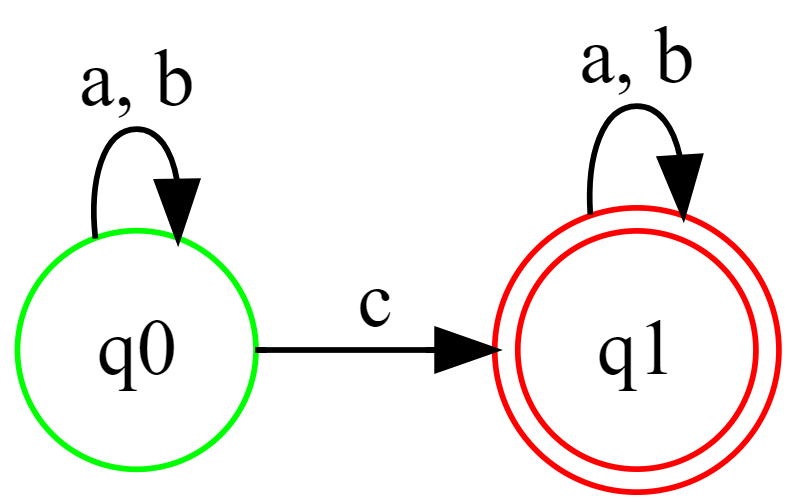
\includegraphics[width=7cm]{Задание_№1_1.png}
\end{figure}

\item {$L = \{ w \in \{a,b\}^*$ | $  {|w|_a} \le 2, {|w|_b} \ge 2 \}$}\\ 
\ У нас может быть 1 или 2 буквы а и бесконечное число букв b, начиная с двух\\
\ Примерные варианты: bb..aa; bab..ba; bab..ab;ab..ab; ab..bb;  и т д  \\
\begin{figure}[h]
\centering
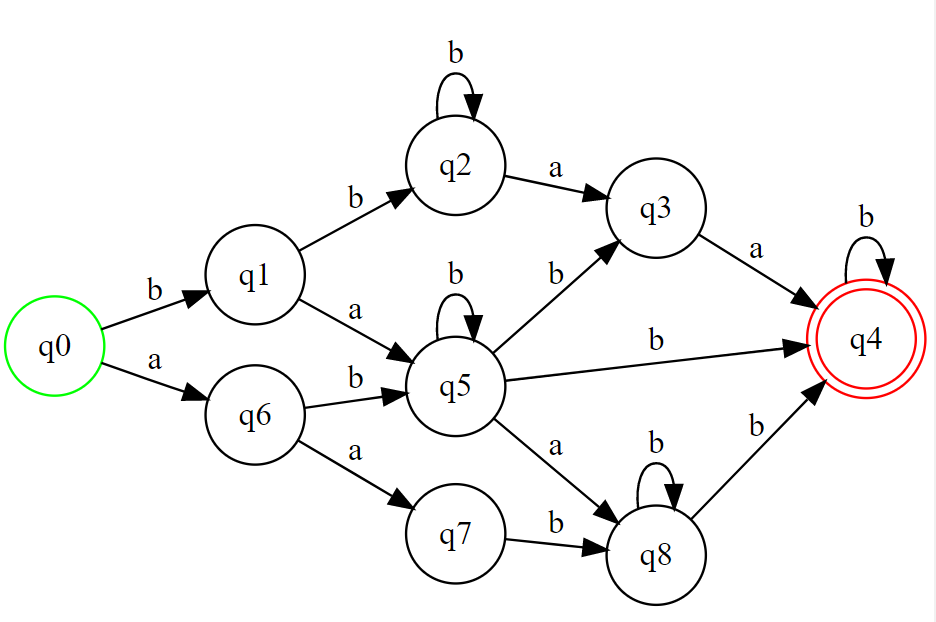
\includegraphics[width=18cm]{Задание_№1_2.png}
\end{figure}
\\Проверим через прямое произведение\\

Построим сначала автомат:\\
$L_1_1 = \{ w \in \{a,b\}  $ | $  {|w|_a} \le 2 \} $\\
\begin{figure}[h]
\centering
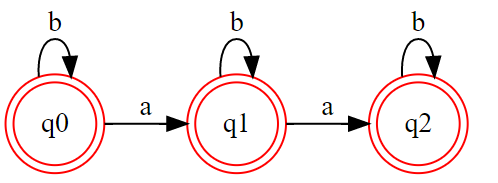
\includegraphics[width=12cm]{Задание_№1_1_2.png}
\end{figure}
\\Потом автомат:\\
$L_1_2 = \{ w \in \{a,b\}  $ | $  {|w|_b} \ge 2 \} $
\begin{figure}[h]
\centering
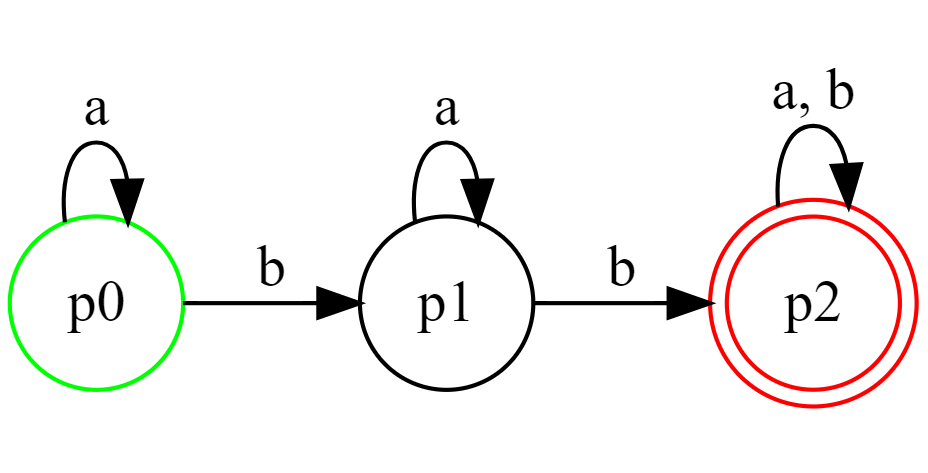
\includegraphics[width=12cm]{Задание_№2_1_1.png}
\end{figure}

\\Найдем ппрямое произведение $L_1_1$ \cap $L_1_2$.
\\где  $A_1_1 = (\sum_1 , Q_1, s_1, T_1, \delta_1) $ и  $A_1_2 = (\sum_2 , Q_2, s_2, T_2, \delta_2)$:\\
\hfill \break
$\sum = \sum_1 \bigcup \sum_2 = \{a, b\}$\\
$Q = Q_1 \times Q_2$ $= \{q0p0, q0p1, q0p2, q1p0, q1p1, q1p2, q2p0, q2p1, q2p2 \}$\\
$s = <s_1, s_2> = q0p0$\\
$T = T_1 \times T_2 = q2p2, q1p2, q0p2$\\
$ \delta(<q1, q2>, c) = <\delta_1(q_1, c), \delta_2(q_2, c)>$\\ Распишем все $\delta$ \\
$\delta(q0p0, a) = q1p0$ \ $\delta(q0p0, b) = q0p1$ \\
$\delta(q0p1, a) = q1p1$ \ $\delta(q0p1, b) = q0p2$ \\
$\delta(q0p2, a) = q1p2$ \ $\delta(q0p2, b) = q0p2$ \\
$\delta(q1p0, a) = q2p0$ \ $\delta(q1p0, b) = q1p1$ \\
$\delta(q1p1, a) = q2p1$ \ $\delta(q1p1, b) = q1p2$ \\
$\delta(q1p2, a) = q2p2$ \ $\delta(q1p2, b) = q1p2$ \\
$\delta(q2p0, a) = -$ \ \ \ \ \ $\delta(q2p0, b) = q2p1$ \\
$\delta(q2p1, a) = -$ \ \ \ \ \ $\delta(q2p1, b) = q2p2$ \\
$\delta(q2p2, a) = -$ \ \ \ \ \ $\delta(q2p2, b) = q2p2$ \\
Построем автомат:\\
\begin{figure}[h]
\centering
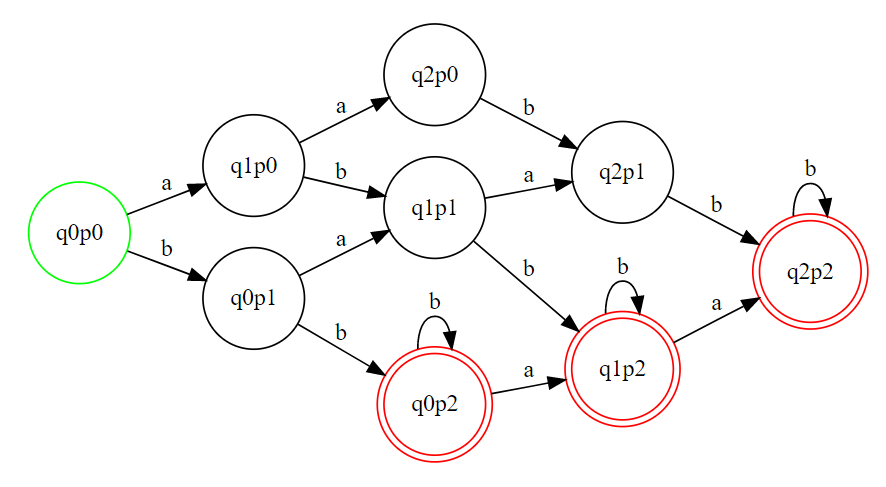
\includegraphics[width=18cm]{Задание_№1_1_3.png}
\end{figure}
\\Заметим, что автоматы не совпадают. Ответом является второй автомат, построенный через прямое произведение
\item {$L = \{ w \in \{a,b\}^*$ | $  {|w|_a} \ne {|w|_b}  \}$} \\
${|w|_a} \ne {|w|_b}$ условно можно заменить на ${|w|_a} > {|w|_b}$ or ${|w|_a} < {|w|_b}$ \\
В случае мы не сможем построить конечный автомат\\

\item {$L = \{ w \in \{a,b\}^*$ | $  {ww = www} \}$} \\
Здесь могут быть только пустые слова 
\begin{figure}[h]
\centering
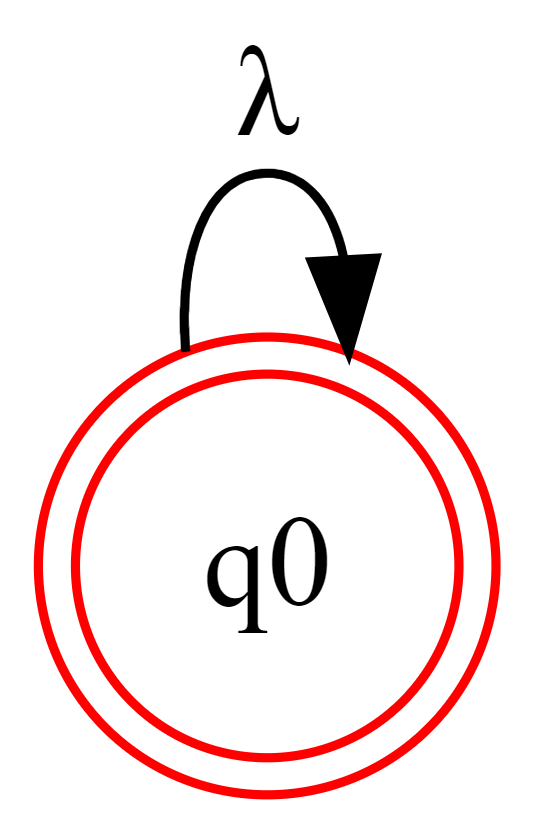
\includegraphics[width=4cm]{Задание_№1_4.png}
\end{figure}
\end{enumerate}
\newpage
% КОНЕЦ ЗАДАНИЯ 1


% ЗАДАНИЕ 2
\newpage
\section{Задание №2. Построить конечный автомат, используя прямое произведение.}
\begin{enumerate}
\item {$L_1 = \{ w \in \{a,b\}  $ | $  {|w|_a} \ge 2  \wedge   {|w|_b} \ge 2 \} $}\\
Построим сначала автомат: 
$L_1_1 = \{ w \in \{a,b\}  $ | $  {|w|_a} \ge 2 \} $
\begin{figure}[h]
\centering
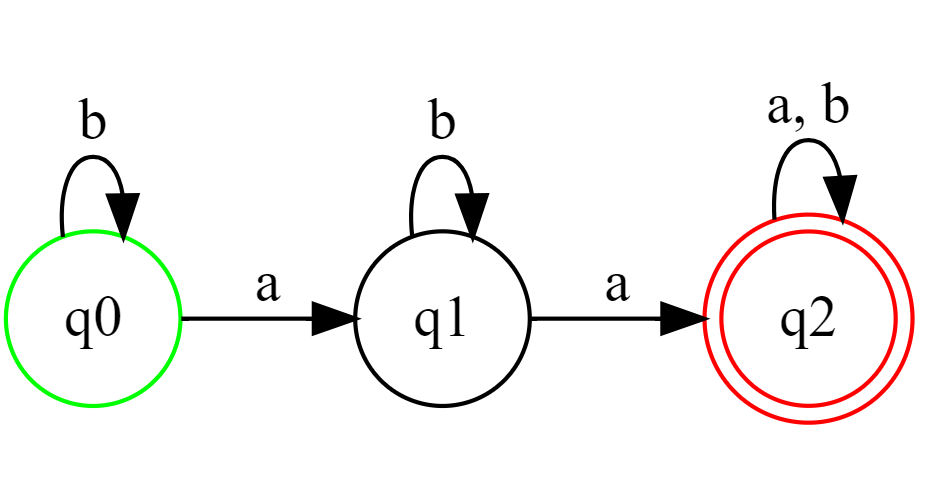
\includegraphics[width=12cm]{Задание_№2_1_2.png}
\end{figure}
\\Потом автомат:
$L_1_2 = \{ w \in \{a,b\}  $ | $  {|w|_b} \ge 2 \} $
\begin{figure}[h]
\centering
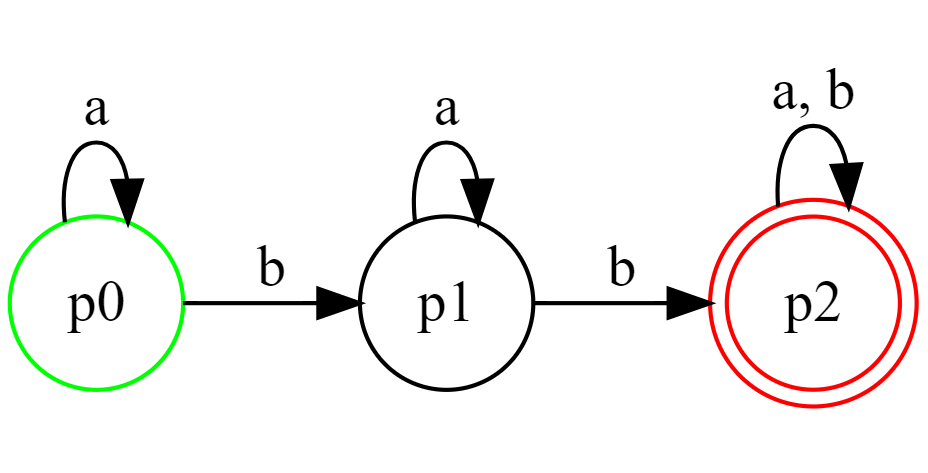
\includegraphics[width=12cm]{Задание_№2_1_1.png}
\end{figure}
\\Найдем ппрямое произведение $L_1_1$ \cap $L_1_2$.
\\где  $A_1_1 = (\sum_1 , Q_1, s_1, T_1, \delta_1) $ и  $A_1_2 = (\sum_2 , Q_2, s_2, T_2, \delta_2)$:\\
\hfill \break
$\sum = \sum_1 \bigcup \sum_2 = \{a, b\}$\\
$Q = Q_1 \times Q_2$ $= \{q0p0, q0p1, q0p2, q1p0, q1p1, q1p2, q2p0, q2p1, q2p2 \}$\\
$s = <s_1, s_2> = q0p0$\\
$T = T_1 \times T_2 = q2p2$\\
$ \delta(<q1, q2>, c) = <\delta_1(q_1, c), \delta_2(q_2, c)>$\\ Распишем все $\delta$ \\
$\delta(q0p0, a) = q1p0$ \  $\delta(q0p0, b) = q0p1$ \\
$\delta(q0p1, a) = q1p1$ \  $\delta(q0p1, b) = q0p2$ \\
$\delta(q0p2, a) = q1p2$ \  $\delta(q0p2, b) = q0p2$ \\
$\delta(q1p0, a) = q2p0$ \  $\delta(q1p0, b) = q1p1$ \\
$\delta(q1p1, a) = q2p1$ \  $\delta(q1p1, b) = q1p2$ \\
$\delta(q1p2, a) = q2p2$ \  $\delta(q1p2, b) = q1p2$ \\
$\delta(q2p0, a) = q2p0$ \  $\delta(q2p0, b) = q2p1$ \\
$\delta(q2p1, a) = q2p1$ \  $\delta(q2p1, b) = q2p2$ \\
$\delta(q2p2, a) = q2p2$ \  $\delta(q2p2, b) = q2p2$ \\
Построим автомат:\\
\begin{figure}[h]
\centering
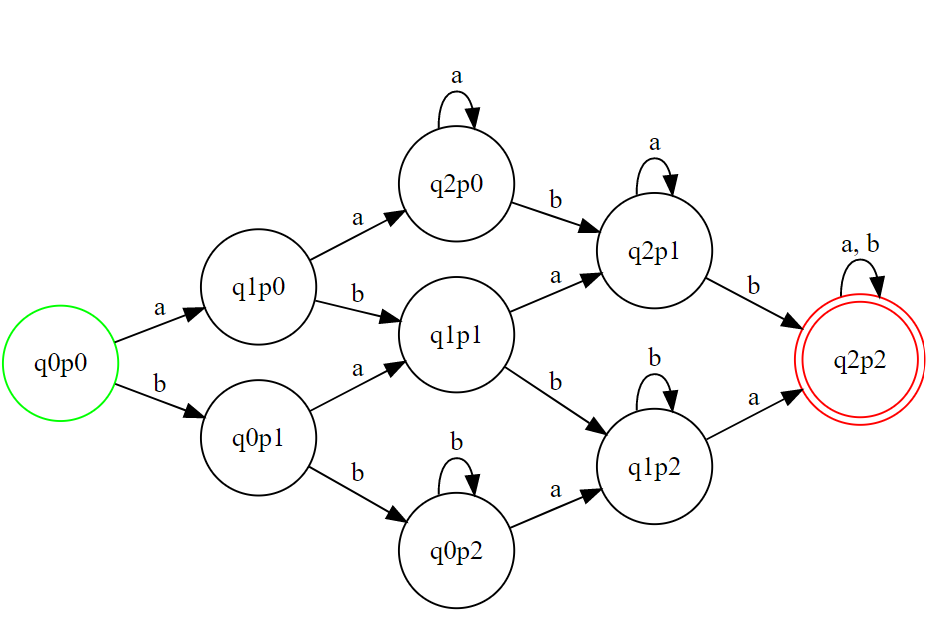
\includegraphics[width=18cm]{Задание_№2_1_3.png}
\end{figure}


\item {$L_2 = \{ w \in \{a,b\}^*$ | $  {|w|} \ge 3 \wedge {|w|} $ нечётное $ \} $}\\


Построим сначала автомат: 
$L_1_1$ = \{$ w \in \{a,b\}^*   $|$  {|w|} \ge 3 $ \} \\
\begin{figure}[h]
\centering
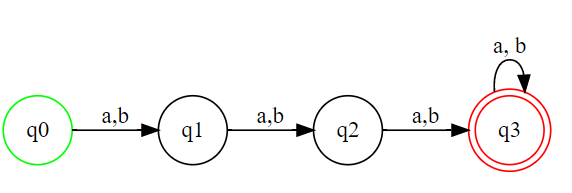
\includegraphics[width=15cm]{Задание_№2_2_1.png}
\end{figure}
\\Потом автомат:
$L_1_2$ = \{$ w \in \{a,b\}^*   $|$  {|w|} $ нечётное $ $ \} \\
Количество вхождений a или b в слово w должно быть нечетным.

\begin{figure}[h]
\centering
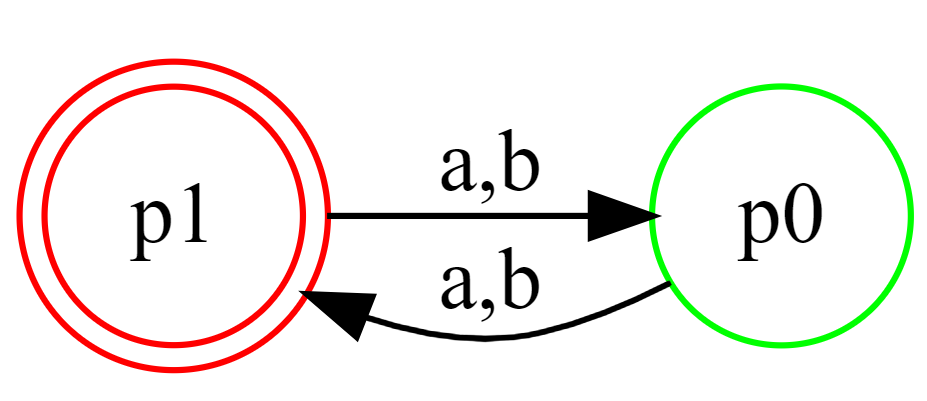
\includegraphics[width=7cm]{Задание_№2_2_2.png}
\end{figure}

\\Найдем прямое произведение $L_1_1$ \cap $L_1_2$.
\\где  $A_1_1 = (\sum_1 , Q_1, s_1, T_1, \delta_1) $ и  $A_1_2 = (\sum_2 , Q_2, s_2, T_2, \delta_2)$:\\
\hfill \break
$\sum = \sum_1 \bigcup \sum_2 = \{a, b\}$\\
$Q = Q_1 \times Q_2$ $= \{q0p0, q0p1, q1p0, q1p1, q2p0, q2p1, q3p0, q3p1 \}$\\
$s = <s_1, s_2> = q0p0$\\
$T = T_1 \times T_2 = q3p1$\\
$ \delta(<q1, q2>, c) = <\delta_1(q_1, c), \delta_2(q_2, c)>$\\ Распишем все $\delta$ \\
$\delta(q0p0, a) = q1p1$ \  $\delta(q0p0, b) = q1p1$ \\
$\delta(q0p1, a) = q1p0$ \  $\delta(q0p1, b) = q1p0$ \\
$\delta(q1p0, a) = q2p1$ \  $\delta(q1p0, b) = q2p1$ \\
$\delta(q1p1, a) = q2p0$ \  $\delta(q1p1, b) = q2p0$ \\
$\delta(q2p0, a) = q3p1$ \  $\delta(q2p0, b) = q3p1$ \\
$\delta(q2p1, a) = q3p0$ \  $\delta(q2p1, b) = q3p0$ \\
$\delta(q3p0, a) = q3p1$ \  $\delta(q3p0, b) = q3p1$ \\
$\delta(q3p1, a) = q3p0$ \  $\delta(q3p1, b) = q3p0$ \\

Построим автомат:\\
\begin{figure}[h]
\centering
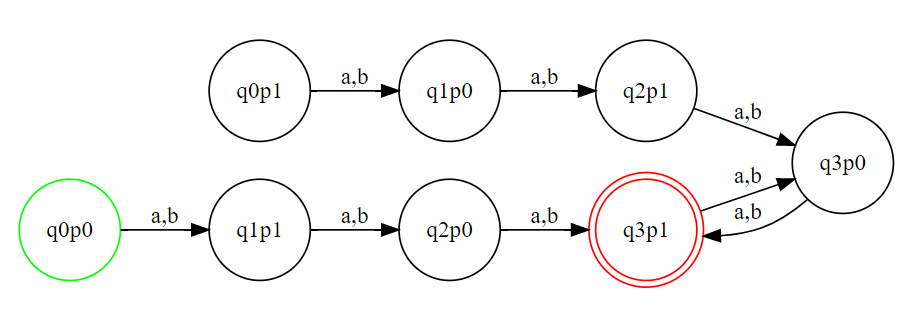
\includegraphics[width=18cm]{Задание_№2_2_3.png}
\end{figure}


\item {$L_3$ = \{ $w$ \in \{$a,b$\}$*$ $|$  $ {|w|_a}$ чётно  $\wedge$ ${|w|_b}$ кратно трём \} }\\
Построим сначала автомат: 
$L_1_1$ = \{$ w \in \{a,b\}*   $|$  {|w|_a} $чётно$ $ \} \\
\begin{figure}[h]
\centering
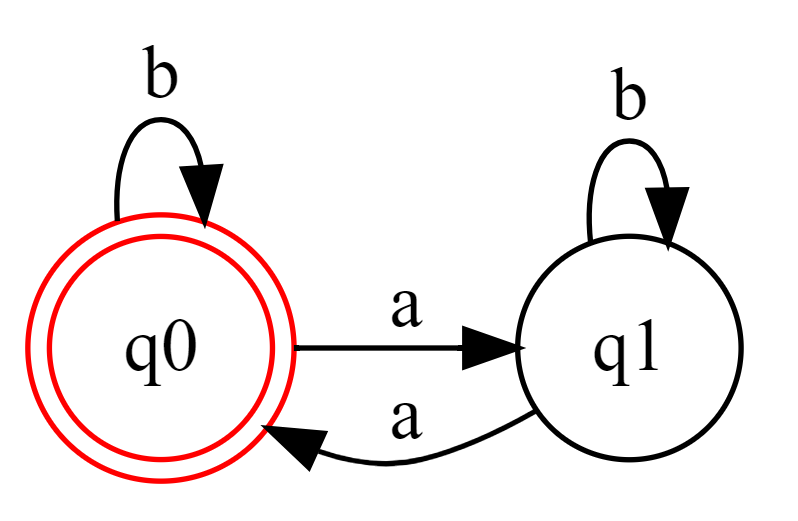
\includegraphics[width=8cm]{Задание_№2_3_1.png}
\end{figure}
\\
\\Потом автомат:
$L_1_2$ = \{$ w \in \{a,b\}*   $|$  {|w|_b} $ кратно трём $ $ \} \\
\begin{figure}[h]
\centering
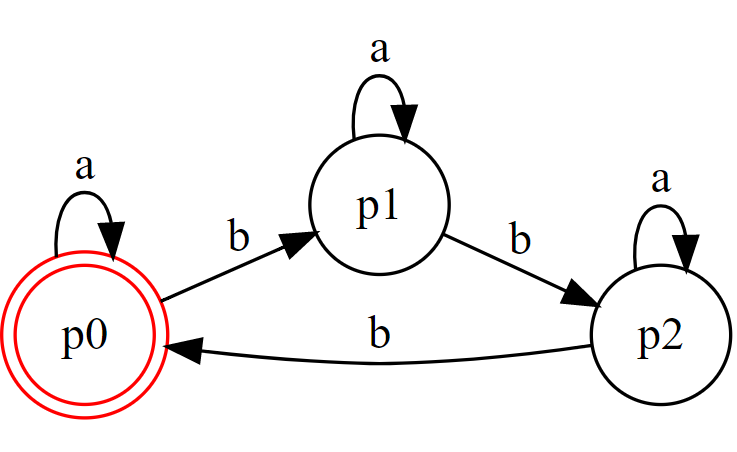
\includegraphics[width=9cm]{Задание_№2_3_2.png}
\end{figure}

\\Найдем прямое произведение $L_1_1$ \cap $L_1_2$.
\\где  $A_1_1 = (\sum_1 , Q_1, s_1, T_1, \delta_1) $ и  $A_1_2 = (\sum_2 , Q_2, s_2, T_2, \delta_2)$:\\
\hfill \break
$\sum = \sum_1 \bigcup \sum_2 = \{a, b\}$\\
$Q = Q_1 \times Q_2$ $= \{q0p0, q0p1, q0p2, q1p0, q1p1, q1p2 \}$\\
$s = <s_1, s_2> = q0p0$\\
$T = T_1 \times T_2 = q0p0$\\
$ \delta(<q1, q2>, c) = <\delta_1(q_1, c), \delta_2(q_2, c)>$\\ 
\\Распишем все $\delta$ \\ \\
$\delta(q0p0, a) = q1p0$ \  $\delta(q0p0, b) = q0p1$ \\
$\delta(q0p1, a) = q1p1$ \  $\delta(q0p1, b) = q0p2$ \\
$\delta(q0p2, a) = q1p2$ \  $\delta(q0p2, b) = q0p0$ \\
$\delta(q1p0, a) = q0p0$ \  $\delta(q1p0, b) = q1p1$ \\
$\delta(q1p1, a) = q0p1$ \  $\delta(q1p1, b) = q1p2$ \\
$\delta(q1p2, a) = q0p2$ \  $\delta(q1p2, b) = q1p0$ \\

\\Построим автомат:\\
\begin{figure}[h]
\centering
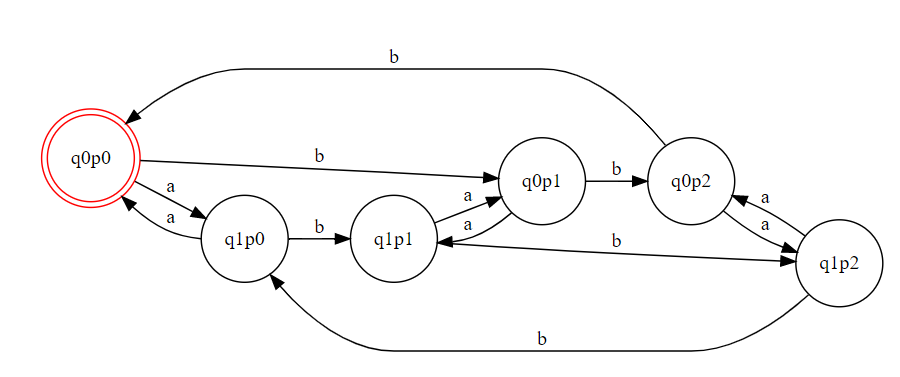
\includegraphics[width=16cm]{Задание_№2_3_3.png}
\end{figure}


\item {$L_4$ = $\overline{L_3}$}\\

$\sum = \sum_1 \bigcup \sum_2 = \{a, b\}$\\
$Q = Q_1 \times Q_2$ $= \{q0p0, q0p1, q0p2, q1p0, q1p1, q1p2 \}$\\
$s = <s_1, s_2> = q0p0$\\
$T = T_1 \times T_2 = q0p1, q0p2, q1p0, q1p1, q1p2 $\\
$ \delta(<q1, q2>, c) = <\delta_1(q_1, c), \delta_2(q_2, c)>$\\ 
\begin{figure}[h]
\centering
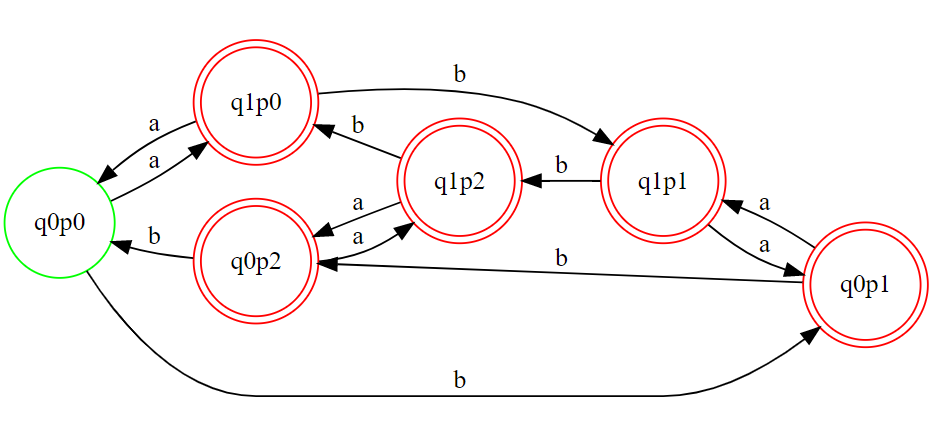
\includegraphics[width=16cm]{Задание_№2_4_1.png}0
\end{figure}
\hfill \break
\item {$L_5 = L_2 \setminus L_3 $}\\
$L_5 = L_2 \setminus L_3 $ $=$ $L_2 \cap \overline{L_3} = L_2 \times  \overline{L_3}$  $=$ $L_2$ \times $L_4$\\
Переименуем автомат $L_2$ и $L_4$\\
$L_2$\\
Не будем упрощать автомат и оставим как есть\\
\hfill \break
\begin{figure}[h]
\centering
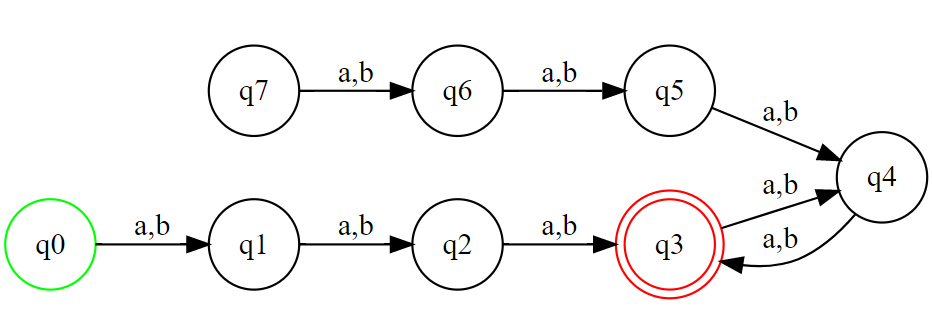
\includegraphics[width=16cm]{Задание_№2_5_1.png}
\end{figure}

$L_4$\\
\hfill \break
\begin{figure}[h]
\centering
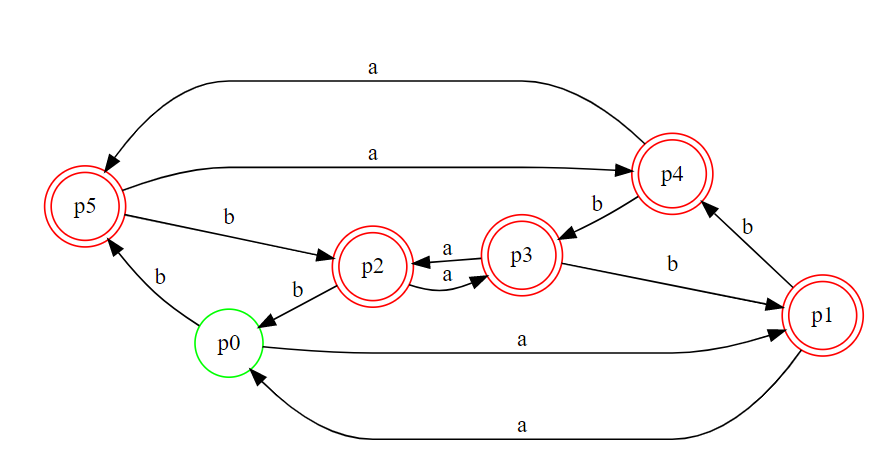
\includegraphics[width=16cm]{Задание_№2_5_2.png}
\end{figure}

\ Тогда:\\
$\sum = \sum_1 \bigcup \sum_2 = \{a, b\}$\\
$Q = Q_1 \times Q_2$ $= \{\\
q0p0, q0p1, q0p2, q0p3, q0p4, q1p5,\\
q1p0, q1p1, q1p2, q1p3, q1p4, q1p5,\\
q2p0, q2p1, q2p2, q2p3, q2p4, q2p5,\\
q3p0, q3p1, q3p2, q3p3, q3p4, q3p5,\\
q4p0, q4p1, q4p2, q4p3, q4p4, q4p5,\\
q5p0, q5p1, q5p2, q5p3, q5p4, q5p5,\\
q0p0, q6p1, q6p2, q6p3, q6p4, q6p5,\\
q7p0, q7p1, q7p2, q7p3, q7p4, q7p5,\\
\}$\\
$s = <s_1, s_2> = q0p0$\\
$T = T_1 \times T_2 = q3p5, q3p2, q3p3, q3p4, q3p1 $\\
$ \delta(<q1, q2>, c) = <\delta_1(q_1, c), \delta_2(q_2, c)>$\\ 
\\Распишем все $\delta$ \\ \\
$\delta(q0p0, a) = q1p1$ \  $\delta(q0p0, b) = q1p5$ \\
$\delta(q0p1, a) = q1p0$ \  $\delta(q0p1, b) = q1p4$ \\
$\delta(q0p2, a) = q1p3$ \  $\delta(q0p2, b) = q1p0$ \\
$\delta(q0p3, a) = q1p2$ \  $\delta(q0p3, b) = q1p1$ \\
$\delta(q0p4, a) = q1p5$ \  $\delta(q0p4, b) = q1p3$ \\
$\delta(q0p5, a) = q1p4$ \  $\delta(q0p5, b) = q1p2$ \\

$\delta(q1p0, a) = q2p1$ \  $\delta(q1p0, b) = q2p5$ \\
$\delta(q1p1, a) = q2p0$ \  $\delta(q1p1, b) = q2p4$ \\
$\delta(q1p2, a) = q2p3$ \  $\delta(q1p2, b) = q2p0$ \\
$\delta(q1p3, a) = q2p2$ \  $\delta(q1p3, b) = q2p1$ \\
$\delta(q1p4, a) = q2p5$ \  $\delta(q1p4, b) = q2p3$ \\
$\delta(q1p5, a) = q2p4$ \  $\delta(q1p5, b) = q2p2$ \\

$\delta(q2p0, a) = q3p1$ \  $\delta(q2p0, b) = q3p5$ \\
$\delta(q2p1, a) = q3p0$ \  $\delta(q2p1, b) = q3p4$ \\
$\delta(q2p2, a) = q3p3$ \  $\delta(q2p2, b) = q3p0$ \\
$\delta(q2p3, a) = q3p2$ \  $\delta(q2p3, b) = q3p1$ \\
$\delta(q2p4, a) = q3p5$ \  $\delta(q2p4, b) = q3p3$ \\
$\delta(q2p5, a) = q3p4$ \  $\delta(q2p5, b) = q3p2$ \\

$\delta(q3p0, a) = q4p1$ \  $\delta(q3p0, b) = q4p5$ \\
$\delta(q3p1, a) = q4p0$ \  $\delta(q3p1, b) = q4p4$ \\
$\delta(q3p2, a) = q4p3$ \  $\delta(q3p2, b) = q4p0$ \\
$\delta(q3p3, a) = q4p2$ \  $\delta(q3p3, b) = q4p1$ \\
$\delta(q3p4, a) = q4p5$ \  $\delta(q3p4, b) = q4p3$ \\
$\delta(q3p5, a) = q4p4$ \  $\delta(q3p5, b) = q4p2$ \\

$\delta(q4p0, a) = q3p1$ \  $\delta(q4p0, b) = q3p5$ \\
$\delta(q4p1, a) = q3p0$ \  $\delta(q4p1, b) = q3p4$ \\
$\delta(q4p2, a) = q3p3$ \  $\delta(q4p2, b) = q3p0$ \\
$\delta(q4p3, a) = q3p2$ \  $\delta(q4p3, b) = q3p1$ \\
$\delta(q4p4, a) = q3p5$ \  $\delta(q4p4, b) = q3p3$ \\
$\delta(q4p5, a) = q3p4$ \  $\delta(q4p5, b) = q3p2$ \\

$\delta(q5p0, a) = q4p1$ \  $\delta(q5p0, b) = q4p5$ \\
$\delta(q5p1, a) = q4p0$ \  $\delta(q5p1, b) = q4p4$ \\
$\delta(q5p2, a) = q4p3$ \  $\delta(q5p2, b) = q4p0$ \\
$\delta(q5p3, a) = q4p2$ \  $\delta(q5p3, b) = q4p1$ \\
$\delta(q5p4, a) = q4p5$ \  $\delta(q5p4, b) = q4p3$ \\
$\delta(q5p5, a) = q4p4$ \  $\delta(q5p5, b) = q4p2$ \\

$\delta(q5p0, a) = q4p1$ \  $\delta(q5p0, b) = q4p5$ \\
$\delta(q5p1, a) = q4p0$ \  $\delta(q5p1, b) = q4p4$ \\
$\delta(q5p2, a) = q4p3$ \  $\delta(q5p2, b) = q4p0$ \\
$\delta(q5p3, a) = q4p2$ \  $\delta(q5p3, b) = q4p1$ \\
$\delta(q5p4, a) = q4p5$ \  $\delta(q5p4, b) = q4p3$ \\
$\delta(q5p5, a) = q4p4$ \  $\delta(q5p5, b) = q4p2$ \\

$\delta(q6p0, a) = q5p1$ \  $\delta(q6p0, b) = q5p5$ \\
$\delta(q6p1, a) = q5p0$ \  $\delta(q6p1, b) = q5p4$ \\
$\delta(q6p2, a) = q5p3$ \  $\delta(q6p2, b) = q5p0$ \\
$\delta(q6p3, a) = q5p2$ \  $\delta(q6p3, b) = q5p1$ \\
$\delta(q6p4, a) = q5p5$ \  $\delta(q6p4, b) = q5p3$ \\
$\delta(q6p5, a) = q5p4$ \  $\delta(q6p5, b) = q5p2$ \\

$\delta(q7p0, a) = q6p1$ \  $\delta(q7p0, b) = q6p5$ \\
$\delta(q7p1, a) = q6p0$ \  $\delta(q7p1, b) = q6p4$ \\
$\delta(q7p2, a) = q6p3$ \  $\delta(q7p2, b) = q6p0$ \\
$\delta(q7p3, a) = q6p2$ \  $\delta(q7p3, b) = q6p1$ \\
$\delta(q7p4, a) = q6p5$ \  $\delta(q7p4, b) = q6p3$ \\
$\delta(q7p5, a) = q6p4$ \  $\delta(q7p5, b) = q6p2$ \\
\begin{figure}[h]
\centering
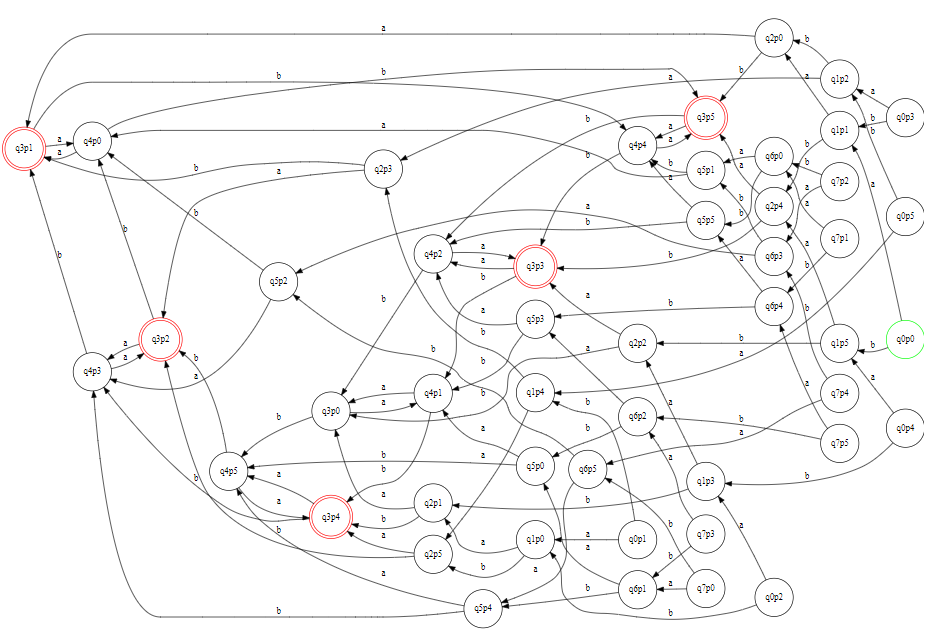
\includegraphics[width=17cm]{Задание_№2_5_3.png}
\end{figure}


\end{enumerate}
\newpage
% КОНЕЦ ЗАДАНИЯ 2

% ЗАДАНИЕ 3
\newpage
\section{Задание №3. Построить минимальные ДКА по регулярному выражению.}
\begin{enumerate}
\item $(ab+aba)^*a$\\
\ У нас есть объединение(+) ab и aba, а затем итерация. \\
\ К сожалению, у меня почему-то не получилось построить красивый автомат, всё съехало. \\
\begin{figure}[h]
\centering
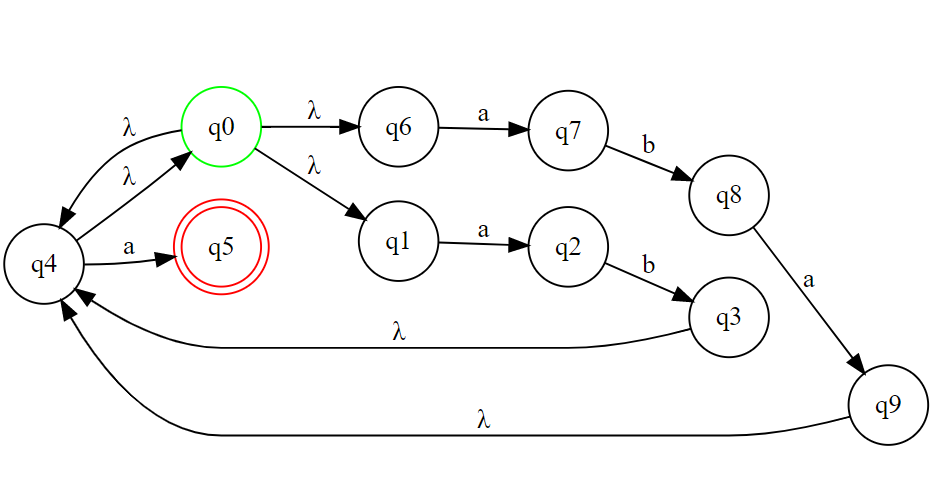
\includegraphics[width=17cm]{Задание_№3_1_1.png}
\end{figure}
\\
\begin{tabular}{|*{3}{c|}}
\textbf{ } & a & b \\
\hline\hline
q0 & q2,q7,q5 & - \\
\hline\hline
q2,q7,q5 & - & q8,q3 \\
\hline\hline
q8,q3 & q9,q5,q2,q7 & - \\
\hline\hline
q9,q5,q2,q7 & q2,q7,q5 & q8,q3 \\
\end{tabular}

\ Тогда построим минимальный ДКА \\
\begin{figure}[h]
\centering
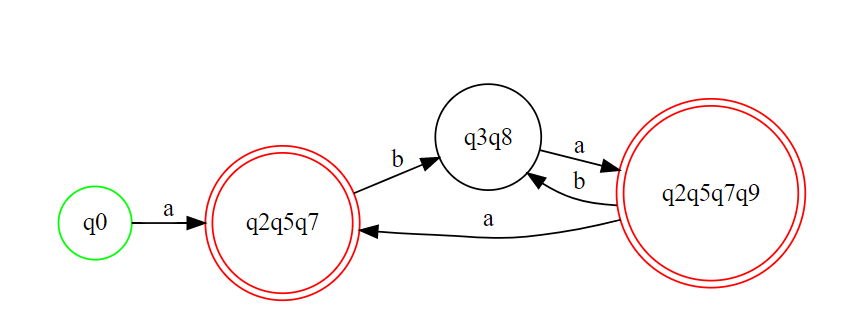
\includegraphics[width=15cm]{Задание_№3_1_2.png}
\end{figure}

\item $a(a(ab)^*b)^*(ab)^*$\\

\begin{figure}[h]
\centering
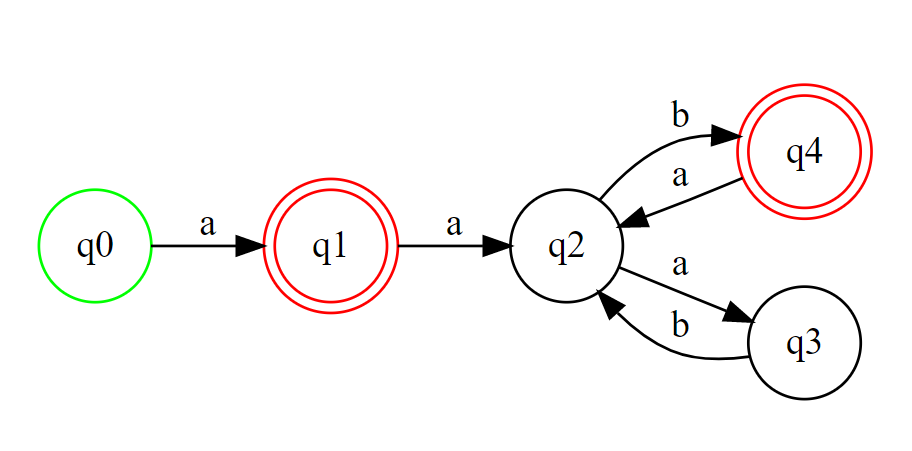
\includegraphics[width=13cm]{Задание_№3_2_1.png}
\end{figure}
\\
\begin{tabular}{|*{3}{c|}}
\textbf{ } & a & b \\
\hline\hline
q0 & q1 & - \\
\hline\hline
q1 & q2 & - \\
\hline\hline
q2 & q3 & q4 \\
\hline\hline
q3 & - & q2 \\
\hline\hline
q4 & q2 & - \\
\end{tabular}
\\Объединим эквивалентные вершины\\

\begin{figure}[h]
\centering
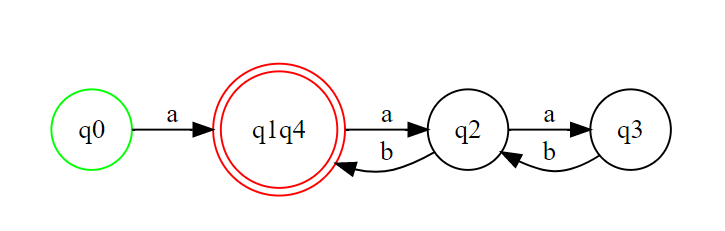
\includegraphics[width=13cm]{Задание_№3_2_2.png}
\end{figure}

\newpage
\item $(a+(a+b)(a+b)b)^*$\\
\\
\begin{figure}[h]
\centering
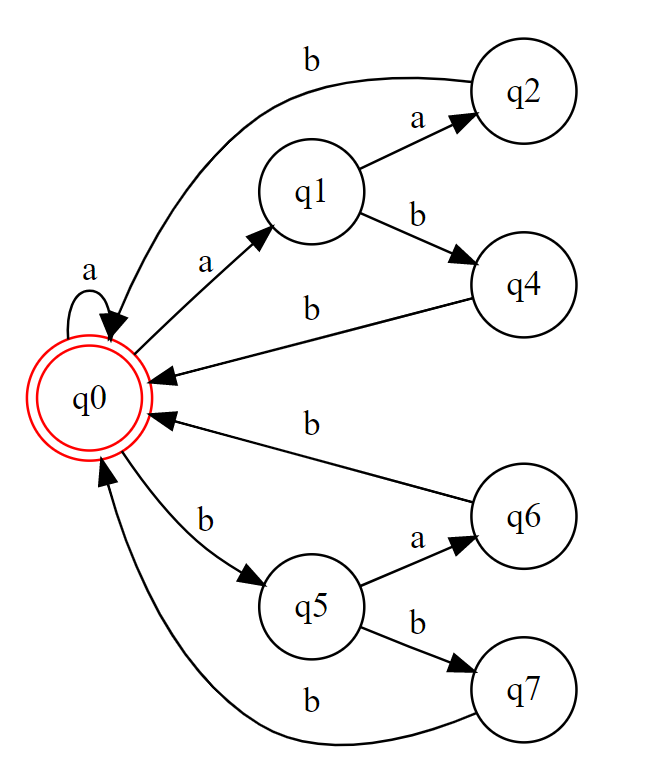
\includegraphics[width=8cm]{Задание_№3_3_1.png}
\end{figure}
\\
\begin{tabular}{|*{3}{c|}}
\textbf{ } & a & b \\
\hline\hline
q0 & q0q1 & q5 \\
\hline\hline
q0q1 & q0q1q2 & q4q5 \\
\hline\hline
q0q1q2 & q0q1q2 & q0q4q5 \\
\hline\hline
q5 & q6 & q7 \\
\hline\hline
q4q5 & q6 & q0q7 \\
\hline\hline
q0q4q5 & q0q1q6 & q0q5q7 \\
\hline\hline
q6 & - & q0 \\
\hline\hline
q7 & - & q0 \\
\hline\hline
q0q7 & q0q1 & q0q5 \\
\hline\hline
q0q5 & q0q1q6 & q5q7 \\
\hline\hline
q5q7 & q6 & q0q7 \\
\hline\hline
q0q1q6 & q0q1q6 & q0q4q5 \\
\hline\hline
q0q5q7 & q0q1q6 & q0q5q7 \\
\end{tabular}
\newpage
Построим минимальный ДКА \\
\begin{figure}[h]
\centering
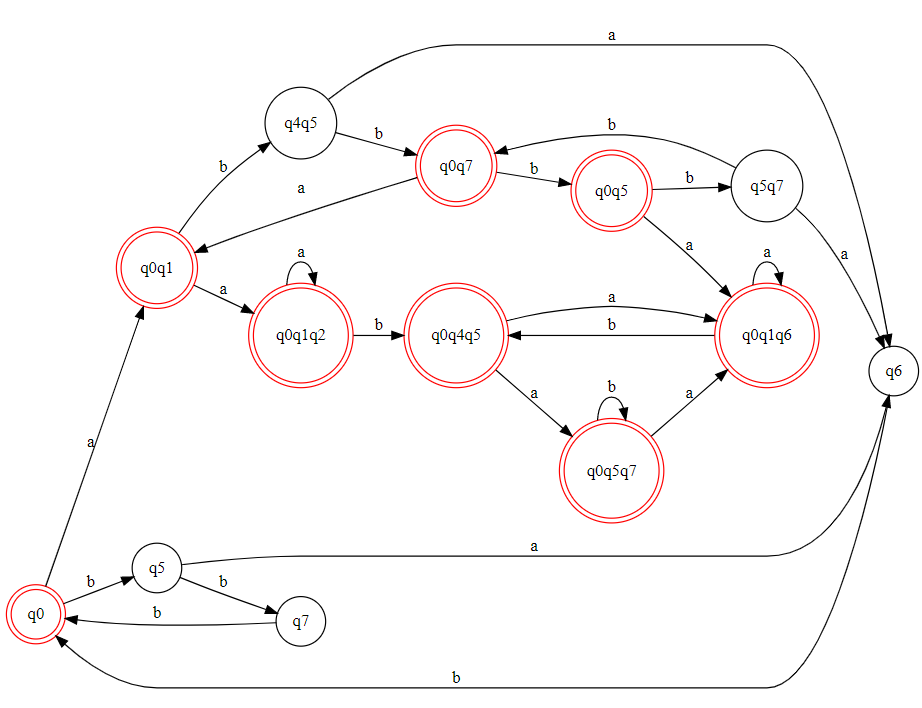
\includegraphics[width=19cm]{Задание_№3_3_2.png}
\end{figure}

Если заменить исходный автомат на эквивалентный, тогда:\\
\begin{figure}[h]
\centering
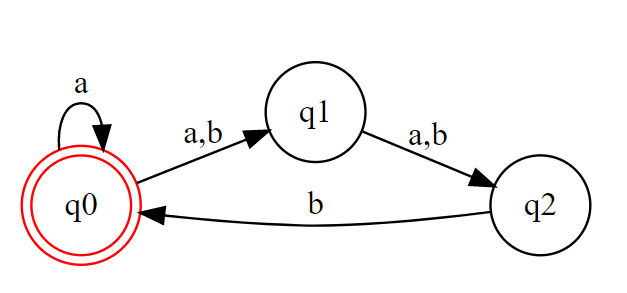
\includegraphics[width=10cm]{Задание_№3_3_3.png}
\end{figure}

\newpage
\begin{tabular}{|*{3}{c|}}
\textbf{ } & a & b \\
\hline\hline
q0 & q0q1 & q1 \\
\hline\hline
q0q1 & q0q1q2 & q1q2 \\
\hline\hline
q0q1q2 & q0q1q2 & q0q1q2 \\
\hline\hline
q1 & q2 & q2 \\
\hline\hline
q2 & - & q0 \\
\hline\hline
q1q2 & q2 & q0q2 \\
\hline\hline
q0q2 & q0q1 & q0q1 \\
\end{tabular}
\\
\\Тогда получим минимальный ДКА \\
\begin{figure}[h]
\centering
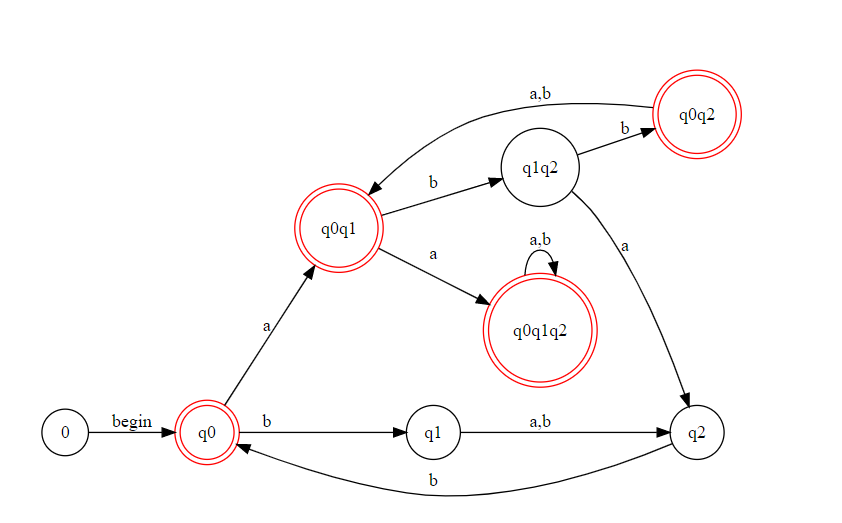
\includegraphics[width=15cm]{Задание_№3_3_4.png}
\end{figure}

\newpage
\item $(b+c)((ab)^*c+(ba)^*)^*$\\
\begin{figure}[h]
\centering
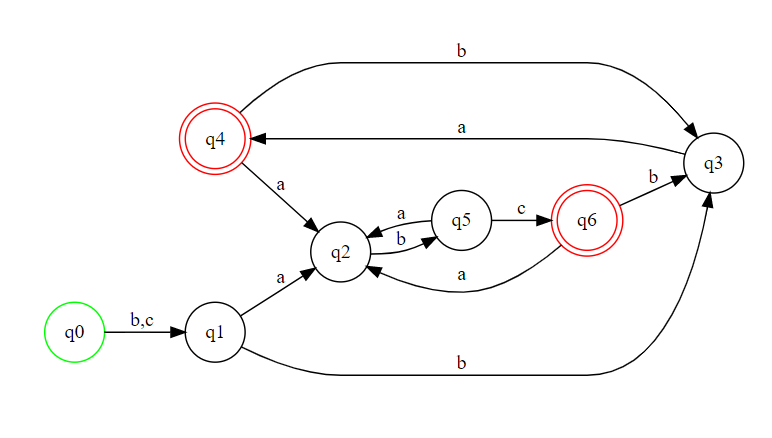
\includegraphics[width=15cm]{Задание_№3_4_1.png}
\end{figure}

\begin{tabular}{|*{4}{c|}}
\textbf{ } & a & b & c\\
\hline\hline
q0 & - & q1 & q1 \\
\hline\hline
q1 & q2 & q3 & - \\
\hline\hline
q2 & - & q5 & - \\
\hline\hline
q3 & q4 & - & - \\
\hline\hline
q4 & q2 & q3 & - \\
\hline\hline
q5 & q2 & - & q6 \\
\hline\hline
q6 & q2 & q3 & - \\
\end{tabular}
\\

\\Вершины q4 и q6 эквивалентны, объединим их\\
\begin{figure}[h]
\centering
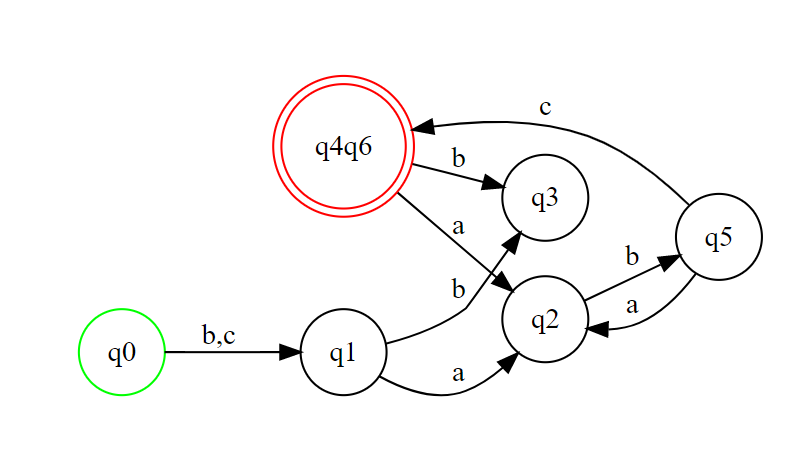
\includegraphics[width=15cm]{Задание_№3_4_2.png}
\end{figure}


\item $(a+b)^+ (aa+bb+abab+baba)(a+b)^+$\\
\begin{figure}[h]
\centering
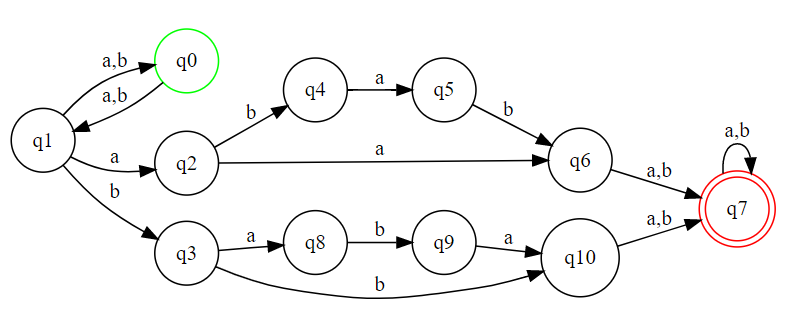
\includegraphics[width=15cm]{Задание_№3_5_1.png}
\end{figure}

\begin{tabular}{|*{3}{c|}}
\textbf{ } & a & b\\
\hline\hline
q0 & q1 & q1 \\
\hline\hline
q1 & q0q2 & q0q3 \\
\hline\hline
q0q2 & q1q6 & q1q4 \\
\hline\hline
q0q3 & q1q8 & q1q10 \\
\hline\hline
q1q6 & q0q2q7 & q0q3q7 \\
\hline\hline
q1q4 & q0q2q5 & q0q3 \\
\hline\hline
q1q8 & q0q2 & q0q3q9 \\
\hline\hline
q1q10 & q0q2q7 & q0q3q7 \\
\hline\hline
q0q2q7 & q1q6q7 & q1q4q7 \\
\hline\hline
q0q3q7 & q1q7q8 & q1q7q10 \\
\hline\hline
q0q2q5 & q1q6 & q1q4q6 \\
\hline\hline
q0q3q9 & q1q8q10 & q1q10 \\
\hline\hline
q1q6q7 & q0q2q7 & q0q3q7 \\
\hline\hline
q1q4q7 & q0q2q5q7 & q0q3q7 \\
\hline\hline
q1q7q8 & q0q2q7 & q0q3q7q9 \\
\hline\hline
q1q7q10 & q0q2q7 & q0q3q7 \\
\hline\hline
q1q4q6 & q0q2q7 & q0q3q7 \\
\hline\hline
q1q8q10 & q0q2q7 & q0q3q9q7 \\
\hline\hline
q0q2q5q7 & q1q6q7 & q1q4q6q7 \\
\hline\hline
q0q3q7q9 & q1q8q7q10 & q1q10q7 \\
\hline\hline
q1q4q6q7 & q0q2q5q7 & q0q3q7 \\
\hline\hline
q1q8q7q10 & q0q2q7 & q0q3q7q9 \\

\end{tabular}
\\

\begin{figure}[h]
\centering
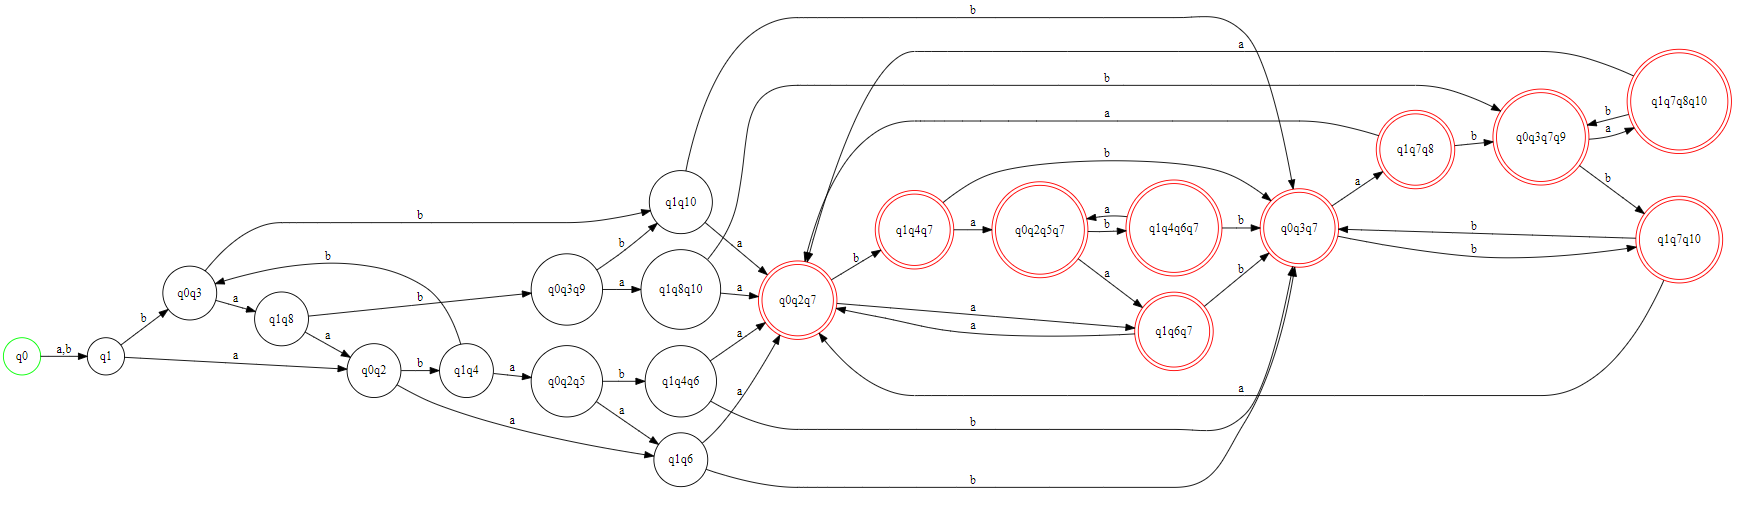
\includegraphics[width=19cm]{Задание_№3_5_2.png}
\end{figure}
\\Найдем эквивалентные вершины\\
\\Все конечные вершины эквивалентны - т е вершины q0q2,q1q4q7,q0q2q5q7,q1q6q7,\\q1q4q6q,q0q3q7
,q1q7q8,q0q3q7q9,q1q7q8q10,q1q7q10 эквиваленты\\
\\Объединим их в одну и обозначим p1\\
\begin{figure}[h]
\centering
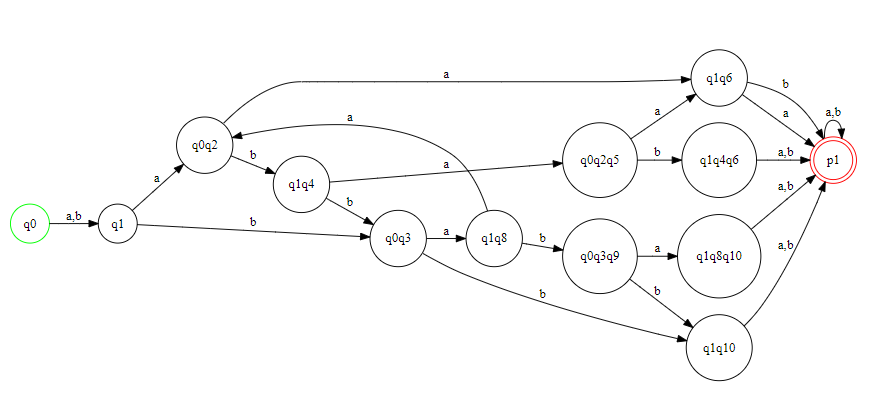
\includegraphics[width=19cm]{Задание_№3_5_3.png}
\end{figure}
\hfill \break
Заметим, что вершины q1q8q10, q1q10 являются эквивалентными, объединим их и обозначим как p2\\
q1q6 и q1q4q6 являются также эквивалентными, объединим их и обозначим как p3\\
\begin{figure}[h]
\centering
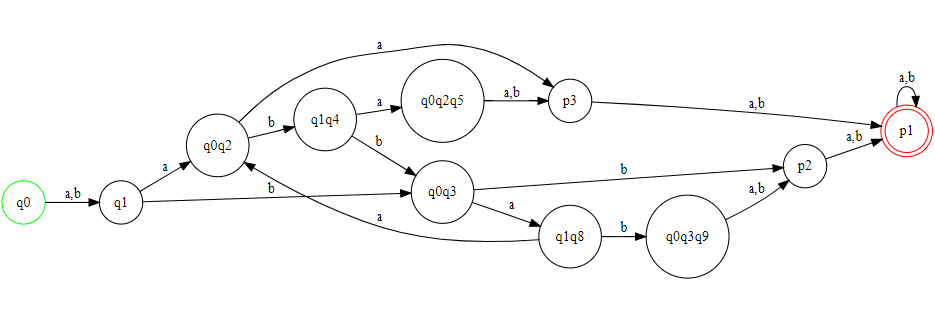
\includegraphics[width=18cm]{Задание_№3_5_4.png}
\end{figure}
\newpage
Не уверена, что так можно, но теперь эквивалентными являются вершины p2 и p3\\
Обозначим их объединение как p4\\

\begin{figure}[h]
\centering
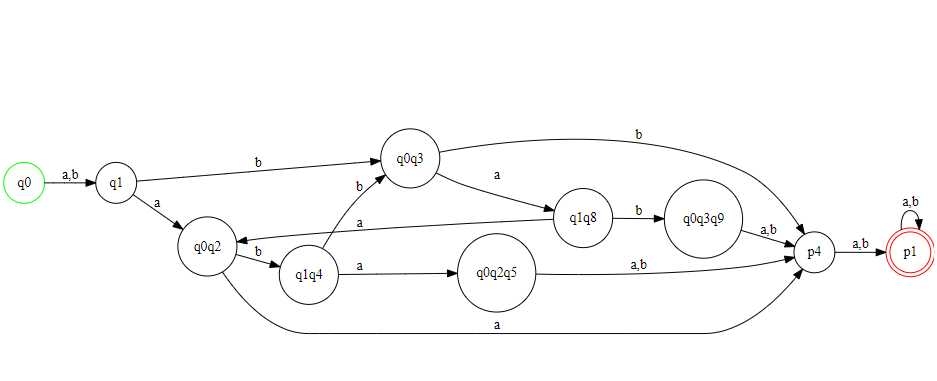
\includegraphics[width=19cm]{Задание_№3_5_5.png}
\end{figure}

\end{enumerate}
\newpage
% КОНЕЦ ЗАДАНИЯ 3


% ЗАДАНИЕ 4
\newpage
\section{Задание №4.Определить является ли язык регулярным или нет.}
\begin{enumerate}
\item $L = \{(aab)^n b(aba)^m  $ | $ $ n \ge 0, m \ge 0 \}

\begin{figure}[h]
\centering
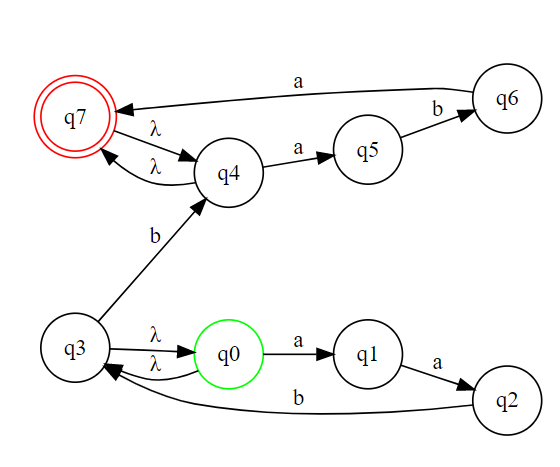
\includegraphics[width=10cm]{Задание_№4_1_1.png}
\end{figure}
\begin{tabular}{|*{4}{c|}}
\textbf{ } & a & b \\
\hline\hline
q0 & q1 & q4  \\
\hline\hline
q1 & q2 & - \\
\hline\hline
q2 & - & q3 \\
\hline\hline
q3 & q1 & q4 \\
\hline\hline
q4 & q5 & - \\
\hline\hline
q5 & - & q6 \\
\hline\hline
q6 & q7 & - \\
\hline\hline
q7 & q5 & - \\
\end{tabular}

\begin{figure}[h]
\centering
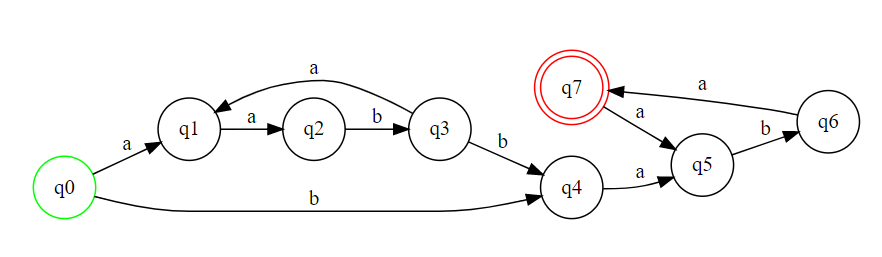
\includegraphics[width=17cm]{Задание_№4_1_2.png}
\end{figure}


\item $L = \{ uaav  | u \in \{a,b\}^* ,  v \in \{a, b\}^* |u|_b\ge|u|_a  \}$
\\ Используем лемму о разрастании\\
Предположим, что язык регулярен. Тогда должна существовать константа n, удовлетворяющая условиям леммы о накачке. Рассмотрим некоторое слово
$w = b^naaa^n, |w| = 2n+2 \ge n.$\\
$w = xyz, |y| \ne 0, |xy| \le n:$\\
$x = b^i, y = b^j, z = b^{n-i-j}aaa^n$\\
$i + j \le n, j \ne 0 $\\
$w = xy^kz=b^ib^{lj}b^{n-i-j}aaa^n$\\
Пусть $l=0,$ тогда: $w = b^{n-j}aaa^n \notin L  ,j \ne 0$\\
Лемма не выполняется => язык не регулярный\\

\item $L = \{ a^mw  | w \in \{a,b\}^* , 1 \le |w|_b \le m   \} $
\\ Используем лемму о разрастании\\
Предположим, что язык регулярен. Тогда должна существовать константа n, удовлетворяющая условиям леммы о накачке. Рассмотрим некоторое слово
$w = a^nb^n, |w| = 2n \ge n.$\\
$w = xyz, |y| \ne 0, |xy| \le n:$\\
$x = a^i, y = a^j, z = a^{n-i-j}b^n$\\
$i + j \le n, j \ne 0 $\\
$w = xy^kz=a^ia^{lj}a^{n-i-j}b^n$\\
Пусть $l=0,$ тогда: $w = a^{n-j}b^n \notin L  ,j \ne 0$\\
Лемма не выполняется => язык не регулярный\\

\item $L = \{ a^kb^ma^n  | k = n \vee m > 0  \} $
\\ Используем лемму о разрастании\\
Предположим, что язык регулярен. Тогда должна существовать константа n, удовлетворяющая условиям леммы о накачке. Рассмотрим некоторое слово
$w = a^nba^n, |w| = 2n+1 \ge n.$\\
$w = xyz, |y| \ne 0, |xy| \le n:$\\
$x = a^i, y = a^j, z = a^{n-i-j}ba^n$\\
$i + j \le n, j \ne 0 $\\
$w = xy^kz=a^ia^{lj}a^{n-i-j}ba^n$\\
Пусть $l=2,$ тогда: $w = a^{n+j}ba^n \notin L  ,j \ne 0$\\
Лемма не выполняется => язык не регулярный\\


\item $L = \{ ucv  | u \in \{a,b\}^*, v \in \{a,b\}^* , u \ne v^R\} $
\\ Используем лемму о разрастании\\
Предположим, что язык регулярен. Тогда должна существовать константа n, удовлетворяющая условиям леммы о накачке.\\ Рассмотрим некоторое слово
\\$w =(ab)^nc(ab)^n = \alpha_1 \alpha_2 ... \alpha_n...\alpha_{2n}...\alpha_{4n}\alpha_{4n+1}, |w| = 4n+1 \ge n.$\\
$w = xyz, |y| \ne 0, |xy| \le n:$\\
$x = \alpha_1 \alpha_2...\alpha_i, y = \alpha_{i+1} \alpha_{i+2}...\alpha_{i+j}, z = \alpha_{i+j+1}\alpha_{i+j+2}...\alpha_{4n+1}c(ab)^n$\\
$i + j \le n, j \ne 0 $\\
$w = xy^lz=(\alpha_1 \alpha_2...\alpha_i)(\alpha_{i+1} \alpha_{i+2}...\alpha_{i+j})^l(\alpha_{i+j+1}\alpha_{i+j+2}...\alpha_{4n+1}c(ab)^n)$\\
\\
Пусть $l=2,$ тогда: $w = (\alpha_1 \alpha_2...\alpha_i)(\alpha_{i+1} \alpha_{i+2}...\alpha_{i+j})^2(\alpha_{i+j+1}\alpha_{i+j+2}...\alpha_{4n+1}c(ab)^n) \notin L  ,j \ne 0$\\
Лемма не выполняется => язык не регулярный\\


\end{enumerate}
\newpage
% КОНЕЦ ЗАДАНИЯ 4

\end{document}  % КОНЕЦ ДОКУМЕНТА !


